\begin{figure*}[!tbh]
    \centering
    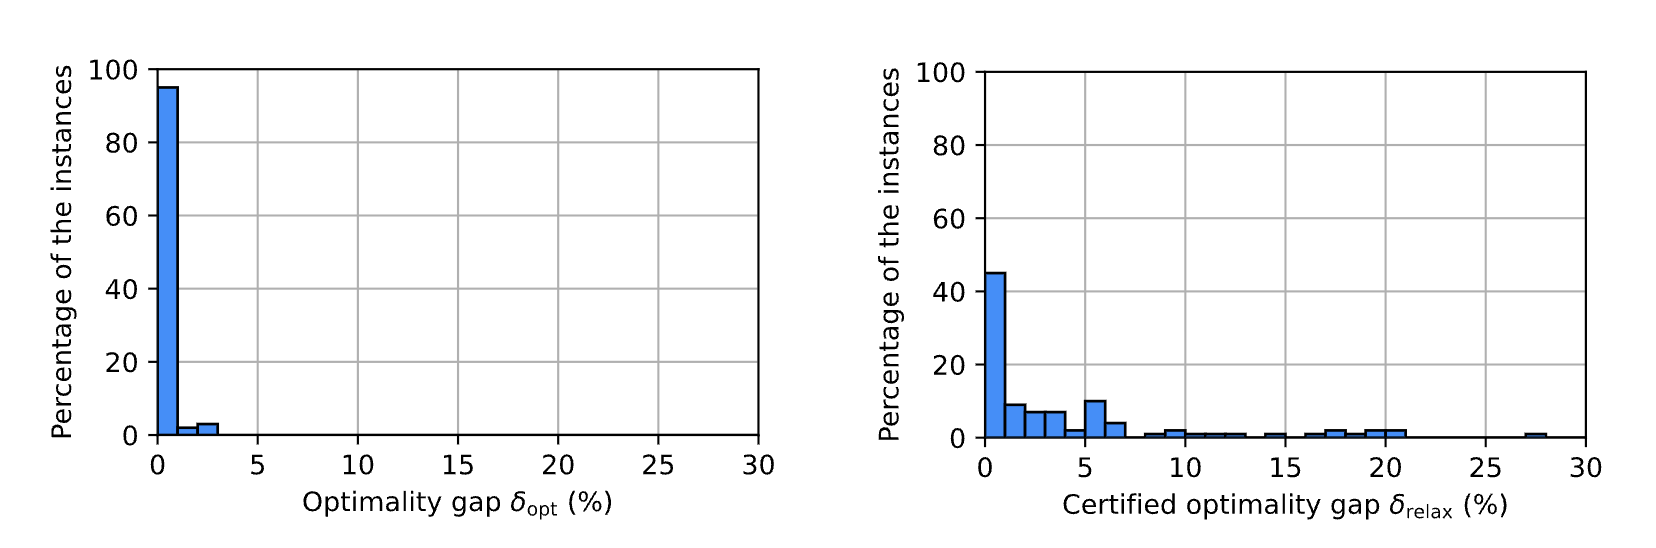
\includegraphics[width=0.8\textwidth]{figures/optimality_gap.png}
    \captionsetup{justification=centering}
    \caption{ {\color{red} todo: replace with real figure after running experiments} }
    \label{fig:}
\end{figure*}

\section{Simulation Results}\label{sec:results}

\subsection{Implementation details}

Our convex optimization-based motion planning approach is primarily built using Drake~\cite{drake}, a widely used toolbox for modeling, simulation and optimization of advanced robotic systems.
We used Drake's implementations of the GCS framework and IRIS to decompose the robot's free configuration space into convex regions.
Note that, to handle the mixed-integer programs generated by the GCS approach, we made use of the MOSEK optimization solver~\cite{mosek}, which supports large scale mixed-integer convex programs.

The robot platform used to validate our approach is a 14-degree-of-freedom dual-arm manipulator as shown in Figure~\ref{fig:simulation}.
The environment we designed resembles a cage, where the robot's task is to move from its initial configuratio---positioned between the first two rows of obstacles---to a goal configuration located between the last two rows of obstacles.
We purposefully constructed this setup to ensure that narrow passages appear in the high-dimensional configuration space of the robot, a known challenge for classical motion planners.
All aspects of the robot's geometry, kinematics and collisions were modeled using Drake's built in simulation and collision checking engines.

{\color{red} \textit{todo: add IRIS details here and the process about how we create and store convex regions}}

In addition to our approach, we use sampling-based motion planners from the Open Motion Planning Library (OMPL)~\cite{sucan2012open} as benchmarks for comparison.
All parameters related to these sampling-based planners were carefully reviewed and adjusted only as necessary to ensure a fair comparison; detailed configurations are omitted from this report.
Interested readers can find more information in our publicly available repository\footnote{\url{https://github.com/utiasSTARS/ece1505-w25-project}}.{\color{red}we should probably move this repo to our own}

\subsection{Analysis}
GCS analysis here

\subsection{Comparison with multi-query planners}

\begin{figure}[!t]
    \centering
    \begin{subfigure}[b]{\linewidth}
        \centering
        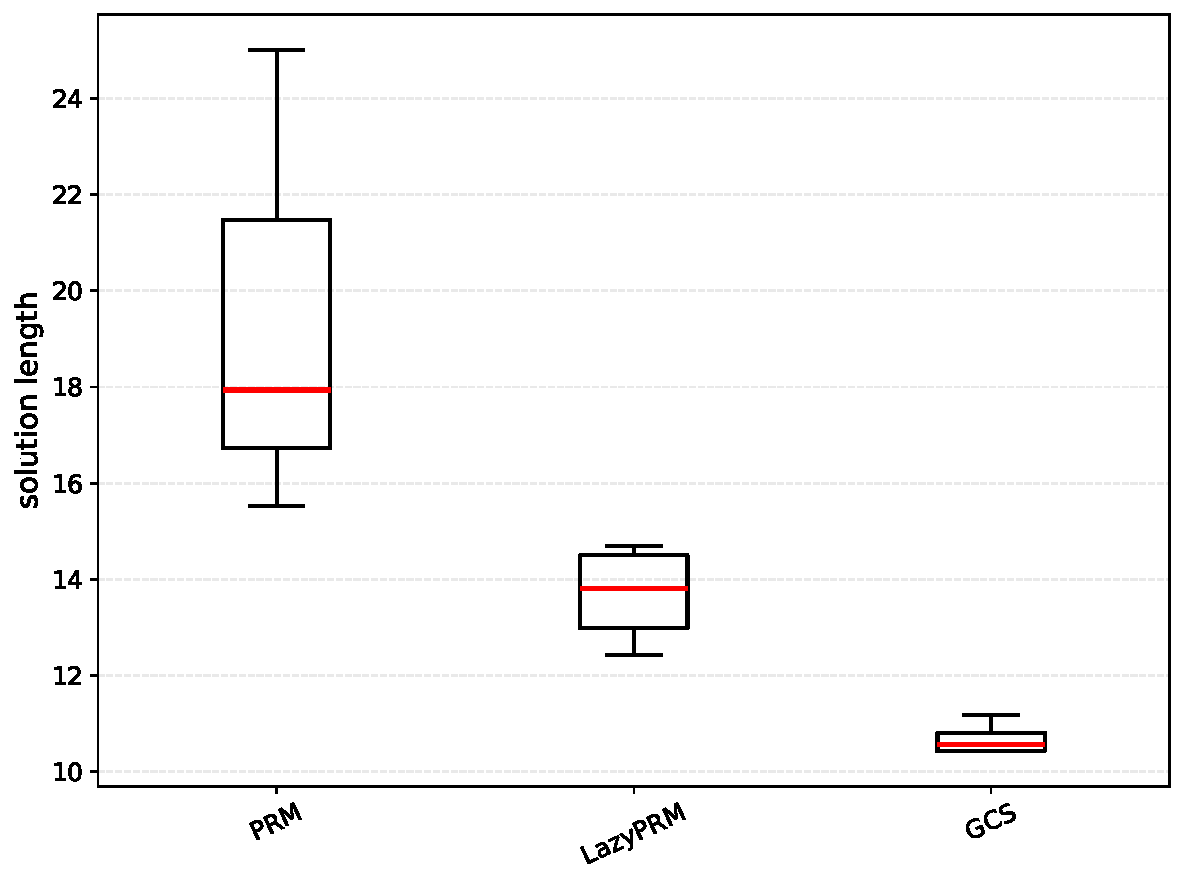
\includegraphics[width=0.8\textwidth]{figures/solution_length_boxplot.pdf}
        \captionsetup{justification=centering}
        % \caption{}
        \label{subfig:}
    \end{subfigure}
    \begin{subfigure}[b]{\linewidth}
        \centering
        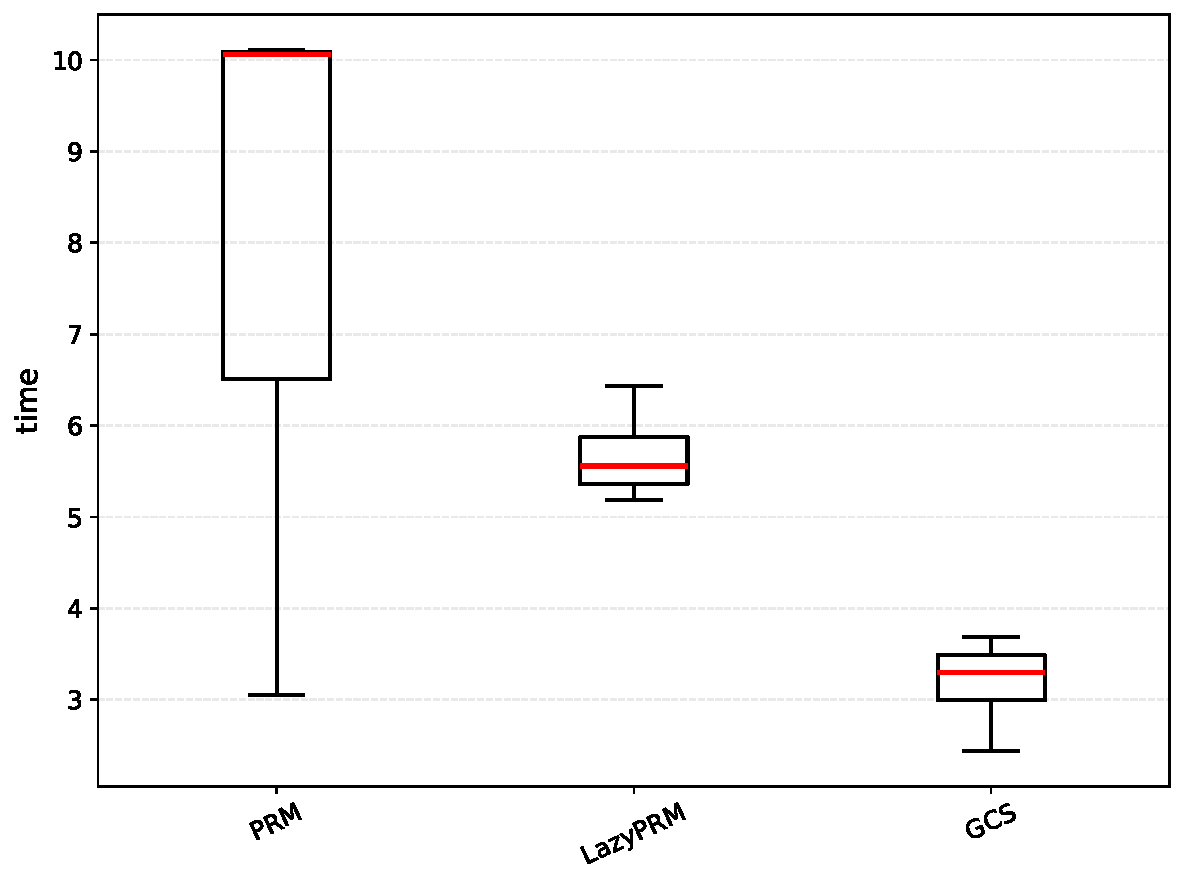
\includegraphics[width=0.8\textwidth]{figures/time_boxplot.pdf}
        \captionsetup{justification=centering}
        % \caption{}
        \label{subfig:}
    \end{subfigure}
    \caption{ {\color{red} todo: update with correct data} }
    \label{fig:}
\end{figure}

% In this experiment, we compare our approach with multi-query sampling-based planners under conditions where precomputation is allowed.
% These planners, such as PRM~\cite{kavraki1996probabilistic} (and its lazy variants~\cite{bohlin2000path}) and Sparse Roadmap Spanners (SPARS)~\cite{dobson2014sparse}, precompute a roadmap (graph) before planning to speed up the solution search.
% We measure metrics such as the time required to find a solution (excluding precomputation), solution quality, and success rate.

\subsection{Comparison with anytime planners}

% We also compare our approach against anytime planners, which can asymptotically improve solution quality over time.
% Specifically, we consider RRT-Connect~\cite{kuffner2000rrt}, BIT*\cite{gammell2020batch}, AIT*\cite{strub2020adaptively}, and Greedy RRT*~\cite{kyaw2024greedy}.
% Here, we focus on how quickly each method finds a solution of comparable quality to ours, as well as its success rate.


